%=============================================================================
%\documentclass[11pt,twoside]{article}
\documentclass[11pt,a4paper,twoside,bibtotoc]{scrartcl}
%\documentclass[twoside,11pt]{article}
%\usepackage{jnm}
%=============================================================================
\usepackage{a4wide}
\usepackage{amsfonts}
\usepackage{amsmath}
\usepackage{theorem}
\usepackage{jkmath}
\usepackage{subfigure}
\usepackage{natbib}
\usepackage{algorithm}
\usepackage{algorithmic}
\usepackage{graphicx}

\theoremstyle{plain}
\newtheorem{theorem}{Theorem}[section]
\newtheorem{corollary}[theorem]{Corollary}
\newtheorem{lemma}[theorem]{Lemma}
\newtheorem{proposition}[theorem]{Proposition}
\theoremstyle{definition}
\newtheorem{definition}[theorem]{Definition}
\newtheorem{example}[theorem]{Example}
\theoremstyle{remark}
\newtheorem{remark}[theorem]{Remark}


\newcommand{\adj}{{\vdash \hspace*{-1.72mm} \dashv}}


\renewcommand{\topfraction}{1}
\renewcommand{\textfraction}{0}
\setcounter{totalnumber}{4}

%============================================================================


\numberwithin{equation}{section}
\numberwithin{table}{section}
\numberwithin{figure}{section}

%\newlength{\temp}
%\setcounter{totalnumber}{10}
%\setcounter{topnumber}{10}

%============================================================================

\title{
%{\rm\normalsize Short Note}\\
Fast Summation on the sphere}

\date{\today}

\author{
Jens Keiner\thanks{keiner@math.uni-luebeck.de, University of
  L\"ubeck, Institute of Mathematics, D--23560 L\"ubeck} \and
Stefan Kunis\thanks{kunis@math.uni-luebeck.de, University of
  L\"ubeck, Institute of Mathematics, D--23560 L\"ubeck} \and
  Daniel Potts\thanks{potts@math.uni-luebeck.de, University of
  L\"ubeck, Institute of Mathematics, D--23560 L\"ubeck} 
}

%=============================================================================
\begin{document}
\maketitle

\begin{abstract}
\medskip

%\noindent
%2000 {\it Mathematics Subject Classification}. 65F10, 65F15, 65T40.

\noindent
{\it Key words and phrases}.  
\end{abstract}

%-----------------------------------------------------------------------------
\section{Introduction}
\label{sect:1}
In radial basis function methods one approximates functions from $\R^3
\rightarrow \R$ by linear combinations of translates of a single function
$\phi:\R^3 \rightarrow \R, \, \phi(x)=\phi(\|x\|_2)$.
The spherical counterpart are the \emph{zonal} functions which depent solely
on the geodesic distance of two points on the sphere $\twosphere:=\{
\V{\xi}: \|\V{\xi}\|_2=1\} \subset \R^3$ and the notion of the former
translation is replaced by the usual inner product.
More formally, let $K \in \Ln{2}{\interv{[}{-1}{1}{]}}$ and define for fixed
$\V{\eta} \in \twosphere$ the $\V{\eta}$-zonal function 
\[
  \fun{K}{\V{\eta} \: \cdot}: \twosphere \rightarrow \R,\ \V{\xi} \mapsto
  \fun{K}{\V{\eta} \cdot \V{\xi}}\,.% \qquad \V{\xi} \in \twosphere.
\]

\section{Prerequisites}
\label{sect:2}
Let the space of real-valued continuous functions on the sphere be decomposed
into the direct sum of spaces of spherical harmonics, i.e.,
$C(\twosphere)=\bigoplus_{k=0}^{\infty} \mathcal{H}_k$, and let
$\set{Y_{k}^n}_{n=-k}^{k}$ denote the standard orthonormal basis of spherical
harmonics.
Using the addition theorem
\[
\sum_{n=-k}^{k} \fun{Y_{k}^n}{\V{\xi}} \overline{\fun{Y_{k}^n}{\V{\eta}}} =
    \frac{2k+1}{4\pi}\fun{P_k}{\V{\eta} \cdot \V{\xi}}
\]
the expansion of the zonal function $\fun{K}{\V{\eta} \: \cdot}$ reduces to
\begin{equation}
  \label{Basics:Kernel}
  \fun{K}{\V{\eta} \cdot \V{\xi}} = \sum_{k = 0}^{\infty} \sum_{n=-k}^k
  \fun{K^{\wedge}}{k}\overline{\fun{Y_{k}^n}{\V{\eta}}} \fun{Y_{k}^n}{\V{\xi}},
\end{equation}
where the \emph{Legendre transform}, i.e. the \emph{symbol} of $K$, is given
for $k \in \NZ$ by
\[
  \fun{K^{\wedge}}{k} := 2 \pi \int_{-1}^{1} \fun{K}{x} \fun{P_{k}}{x} \dx x\,.
\]

\section{Fast Summation}
Given a set of arbitrary \emph{source nodes} $\mathcal{Y} :=
  \pset{\V{\eta}_{l} \in \twosphere}{|}{l = 0,\ldots,L-1}$ and a vector of
  real coefficients $\V{b}:=(b_{l})_{l=0}^{L-1}$, our goal consists in the fast
evaluation of sums 
\begin{equation}
  \label{Applications:KernelSum}
  \fun{f}{\xi} := \sum_{l = 0}^{L-1} b_{l} \fun{K}{\V{\eta}_{l} \cdot \V{\xi}}
\end{equation}
at a set of arbitrary \emph{target nodes} $\mathcal{X} := \pset{\V{\xi}_{d}
  \in \twosphere}{|}{d=0,\ldots,D-1}$.

Given, the zonal function $\fun{K}{\V{\eta} \: \cdot}$ can be evaluated easily
or all the values $\fun{K}{\V{\eta}_{l} \cdot \V{\xi}_{d}}$ can be stored in
advance, the naive approach evaluating \eqref{Applications:KernelSum} leads to
an $\bigo{L\:D}$ algorithm. 
For large $L$ and $D$ the computational effort becomes quickly unaffordable.
The \emph{panel clustering} method introduced in \cite{FrGlSch98} reduces the
computational effort to evaluate \eqref{Applications:KernelSum} based on the
traditional method of dividing the evaluation into near- and far-field.
For every kernel $\fun{K}{\V{\eta}_l \: \cdot}$, the near-field contribution
is calculated exactly whereas the contribution of the far-field may be
approximated coarsly.
% due to the supposed rapid decay of $\fun{K}{\V{\eta} \:\cdot}$. 

We propose to simply truncate the series of the function
$\fun{K}{\V{\eta}_{l}\: \cdot}$ with a degree $M \in \NZ$, i.e.,
\begin{equation}
  \label{Applications:TruncatedSeries}
  \fun{K}{\V{\eta}_{l} \cdot \V{\xi}} \approx \fun{K_{M}}{\V{\eta}_{l} \cdot
  \V{\xi}} := \sum_{k=0}^{M} \sum_{n=-k}^k \fun{K^{\wedge}}{k}
  \fun{Y_{k}^n}{\V{\xi}} \overline{\fun{Y_{k}^n}{\V{\eta}_{l}}}.
\end{equation}

Substituting \eqref{Applications:TruncatedSeries} into
\eqref{Applications:KernelSum} and interchanging the summation order we obtain
our final approximation
\[
  \fun{f_{M}}{\xi_{d}} := \sum_{k=0}^{M} \sum_{n=-k}^k \fun{K^{\wedge}}{k}
  \paren{\sum_{l = 0}^{L-1} b_{l} \overline{\fun{Y_{k}^n}{\V{\eta}_{l}}}}
  \fun{Y_{k}^n}{\V{\xi}_{d}}.
\]

The expression in the inner brackets can be computed by an adjoint Nonuniform
Fast Spherical Fourier Transform (NFSFT) in $\mathcal{O}(L + M^2 \log^2 M)$
arithmetic operations, see \cite{} and the forthcoming paper \cite{} for
details.
This is followed by $(M+1)^2$ multiplications with the symbol
$\fun{K^{\wedge}}{k}$, and completed by a NFSFT to compute the outer sum in
$\mathcal{O}(D + M^2 \log^2 M)$ arithmetic operations.
In Section \ref{Basics:SphericalKernels}, we will decompose the error and show
that the degree $M$ depends only on the desired accuracy of our algorithm and
on the particular zonal function $\fun{K}{\V{\eta} \: \cdot}$, but not on the
numbers $L$ and $D$.
Thus, the overall arithmetic complexity of our algorithm is $\mathcal{O}(L +
D)$, in particular this performance does not depend on the distribution of the
nodes $\V{\xi}_{d}$ and $\V{\eta}_{l}$.

\begin{remark}
In matrix-vector notation the proposed approach, a particular rank $(M+1)^2$
approximation, is given by
\[
  \V{f} = \V{Y_{\mathcal{X}}} \: \V{\hat W} \:
  \V{Y_{\mathcal{Y}}}^{\adj} \: \V{b}
\]
with
\begin{align}
  \nonumber
  \V{f} & := \paren{\fun{f}{\V{\xi}_{d}}}_{d=0}^{D-1} \in \R^D,
  \\ \nonumber
  \V{Y_{\mathcal{X}}} & := \paren{\fun{Y_k^n}{\V{\xi}_{d}}}_{d=0,\ldots,D-1;
  k=0,\ldots,M,\:n=-k,\ldots,k} \in \C^{D \times
  \paren{M+1}^2}, \\ \nonumber
  \V{\hat W} & := \fun{\diag}{\V{\hat w}},\ \V{\hat w} := \paren{\hat
  w_{k}^{n}}_{k=0,\ldots,M,\:n=-k,\ldots,k} \in \R^{(M+1)^2},\ \hat w_{k}^n :=
  \fun{K^{\wedge}}{k}, \\ \nonumber
  \V{Y_{\mathcal{Y}}} & := \paren{\fun{Y_k^n}{\V{\eta}_{l}}}_{l=0,\ldots,L-1;
  k=0,\ldots,M,\:n=-k,\ldots,k} \in \C^{L \times \paren{M+1}^2}.
\end{align}

Replacing the NFSFT by its slow version, which takes $\mathcal{O}(L M^2)$ and
$\mathcal{O}(D M^2)$ arithmetic operations, respectively, yields an
$\mathcal{O}(L+M)$ algorithm, too.
\end{remark}

In summary, we propose the following algorithm.
\begin{algorithm}[h]
  \caption{Fast Summation}
  \label{Applications:Algorithm:FastSummation}    
  \begin{algorithmic}
    \STATE  Input:  $L \in \N$, $\paren{b_{l}}_{l=0}^{L-1}$, $\paren{\V{\eta}_{l}}_{l=0}^{L-1}$, 
                    $D \in \N$, $\paren{\V{\xi}_{d}}_{d=0}^{D-1}$, $M \in \NZ, \paren{\fun{K^{\wedge}}{k}}_{k=0}^M$
    \STATE
    \STATE Compute $\V{\tilde{b}}= \V{Y_{\mathcal{Y}}}^{\adj} \: \V{b}$ by an
                    adjoint NFSFT 
    \STATE 
    \FOR {$k=0,\ldots,M$} 
      \FOR {$n=-k,\ldots,k$} 
        \STATE Set $a_{k}^n = \tilde{b}_{k}^n \: \fun{K^{\wedge}}{k}$
      \ENDFOR
    \ENDFOR
    \STATE
    \STATE Compute $\V{f} = \V{Y_{\mathcal{X}}} \: \V{a}$ by a NFSFT
    \STATE
    \STATE Output: $\paren{\fun{f}{\V{\xi}_{d}}}_{d=0}^{D-1}$
\end{algorithmic}
\end{algorithm}


\section{Error estimate and examples}
\label{Basics:SphericalKernels}
Due to $\max_{x \in \interv{[}{-1}{1}{]}} \abs{\fun{P_{k}}{x}} = 1$, the
proposed approximation obeys the uniform error estimate
\begin{equation}
  \label{error}
  \left\|f - f_{M}\right\|_{\infty} \le
  \left\|\V{b}\right\|_1 \left\|\fun{\left(K-K_M\right)}{\V{\eta} \: \cdot
  }\right\|_{\infty} \le \left\|\V{b}\right\|_1 \sum_{k>M} \frac{2k+1}{4\pi}
  \abs{\fun{K^{\wedge}}{k}}.
\end{equation}

\begin{example}
We consider the generating series
\begin{equation}
  \label{Basics:GeneratingFunction}
  \fun{\phi}{h} := \sum_{k = 0}^{\infty} h^k \fun{P_k}{x} \quad \paren{x \in \interv{[}{-1}{1}{]}}
\end{equation}
which is absolutely and uniformly convergent for $h \in
\interv{(}{-1}{1}{)}$ with
\begin{equation}
  \label{Basics:Solution}
  \sum_{k = 0}^{\infty} h^k \fun{P_k}{x} = \frac{1}{\sqrt{1-2hx+h^2}}.
\end{equation}
This follows from the ordinary differential equation
\begin{equation}
\label{Basics:DifferentialEquation}
  \paren{1+h^2-2hx}\fun{\phi'}{h} = \paren{x-h}\fun{\phi}{h}
\end{equation}
obtained by differentiation with respect to $h$ and comparing coefficients in line with \eqref{Basics:GeneratingFunction}. Using the initial 
condition $\fun{\phi}{0}=1$ this yields the unique solution \eqref{Basics:Solution} of \eqref{Basics:DifferentialEquation}.
From this result, the identity
\begin{equation}
  \nonumber
  \sum_{k=0}^{\infty} \paren{2k+1} h^k \fun{P_k}{x} =
  \frac{1-h^2}{\paren{1-2hx+h^2}^{3/2}}
\end{equation}
 follows easily. When $h$ is restricted to $\interv{(}{0}{1}{)}$ the function
$Q_{h}:\interv{[}{-1}{1}{]} \rightarrow \R$, with
\begin{equation}
  \label{PoissonKernel}
  \nonumber
  \fun{Q_{h}}{x} := \frac{1}{4\pi} \frac{1-h^2}{\paren{1-2hx+h^2}^{3/2}} \quad \paren{x \in \interv{[}{-1}{1}{]}},
\end{equation}
is called \emph{Poisson kernel}. The symbol $\fun{Q_{h}^{\wedge}}{k}$ is given by 
\[
  \fun{Q_{h}^{\wedge}}{k} = h^k.
\]
We refer to Figure \ref{Basics:Figure:PoissonKernel} 
%and \ref{Basics:Figure:PoissonKernel2}
for a visual impression and mention that the parameter $h$
allows for controlling the concentration of the function's energy around
$x = 1$. The Poisson kernel is a positive function and normalized with
\[
  \int_{\twosphere} \fun{Q_{h}}{\V{\eta} \cdot \V{\xi}} \dx \V{\xi} = 1 \quad \paren{\V{\eta} \in \twosphere}.
\]
Further properties with respect to localization and smoothness are derived in \cite[pp. 112]{frgesc}.
\end{example}

\begin{figure}[tbp]
  \centering
  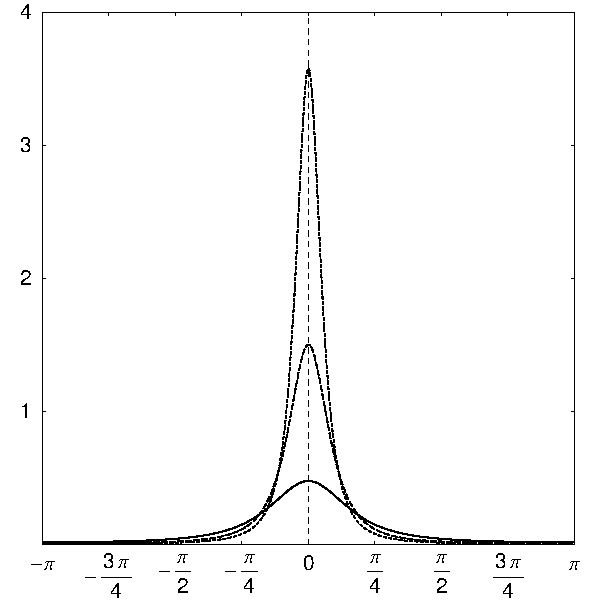
\includegraphics[width=0.7\textwidth]{images/poisson}
  \caption{The Poisson kernel $\fun{Q_{h}}{\cos\theta}$ for $h = 0.5,0.7,0.8$ and $\theta \in \interv{[}{-\pi}{\pi}{]}$.}
  \label{Basics:Figure:PoissonKernel}
\end{figure}

%\begin{figure}[htb]
%  \centering
%   \subfigure[$h=0.70$]
%     {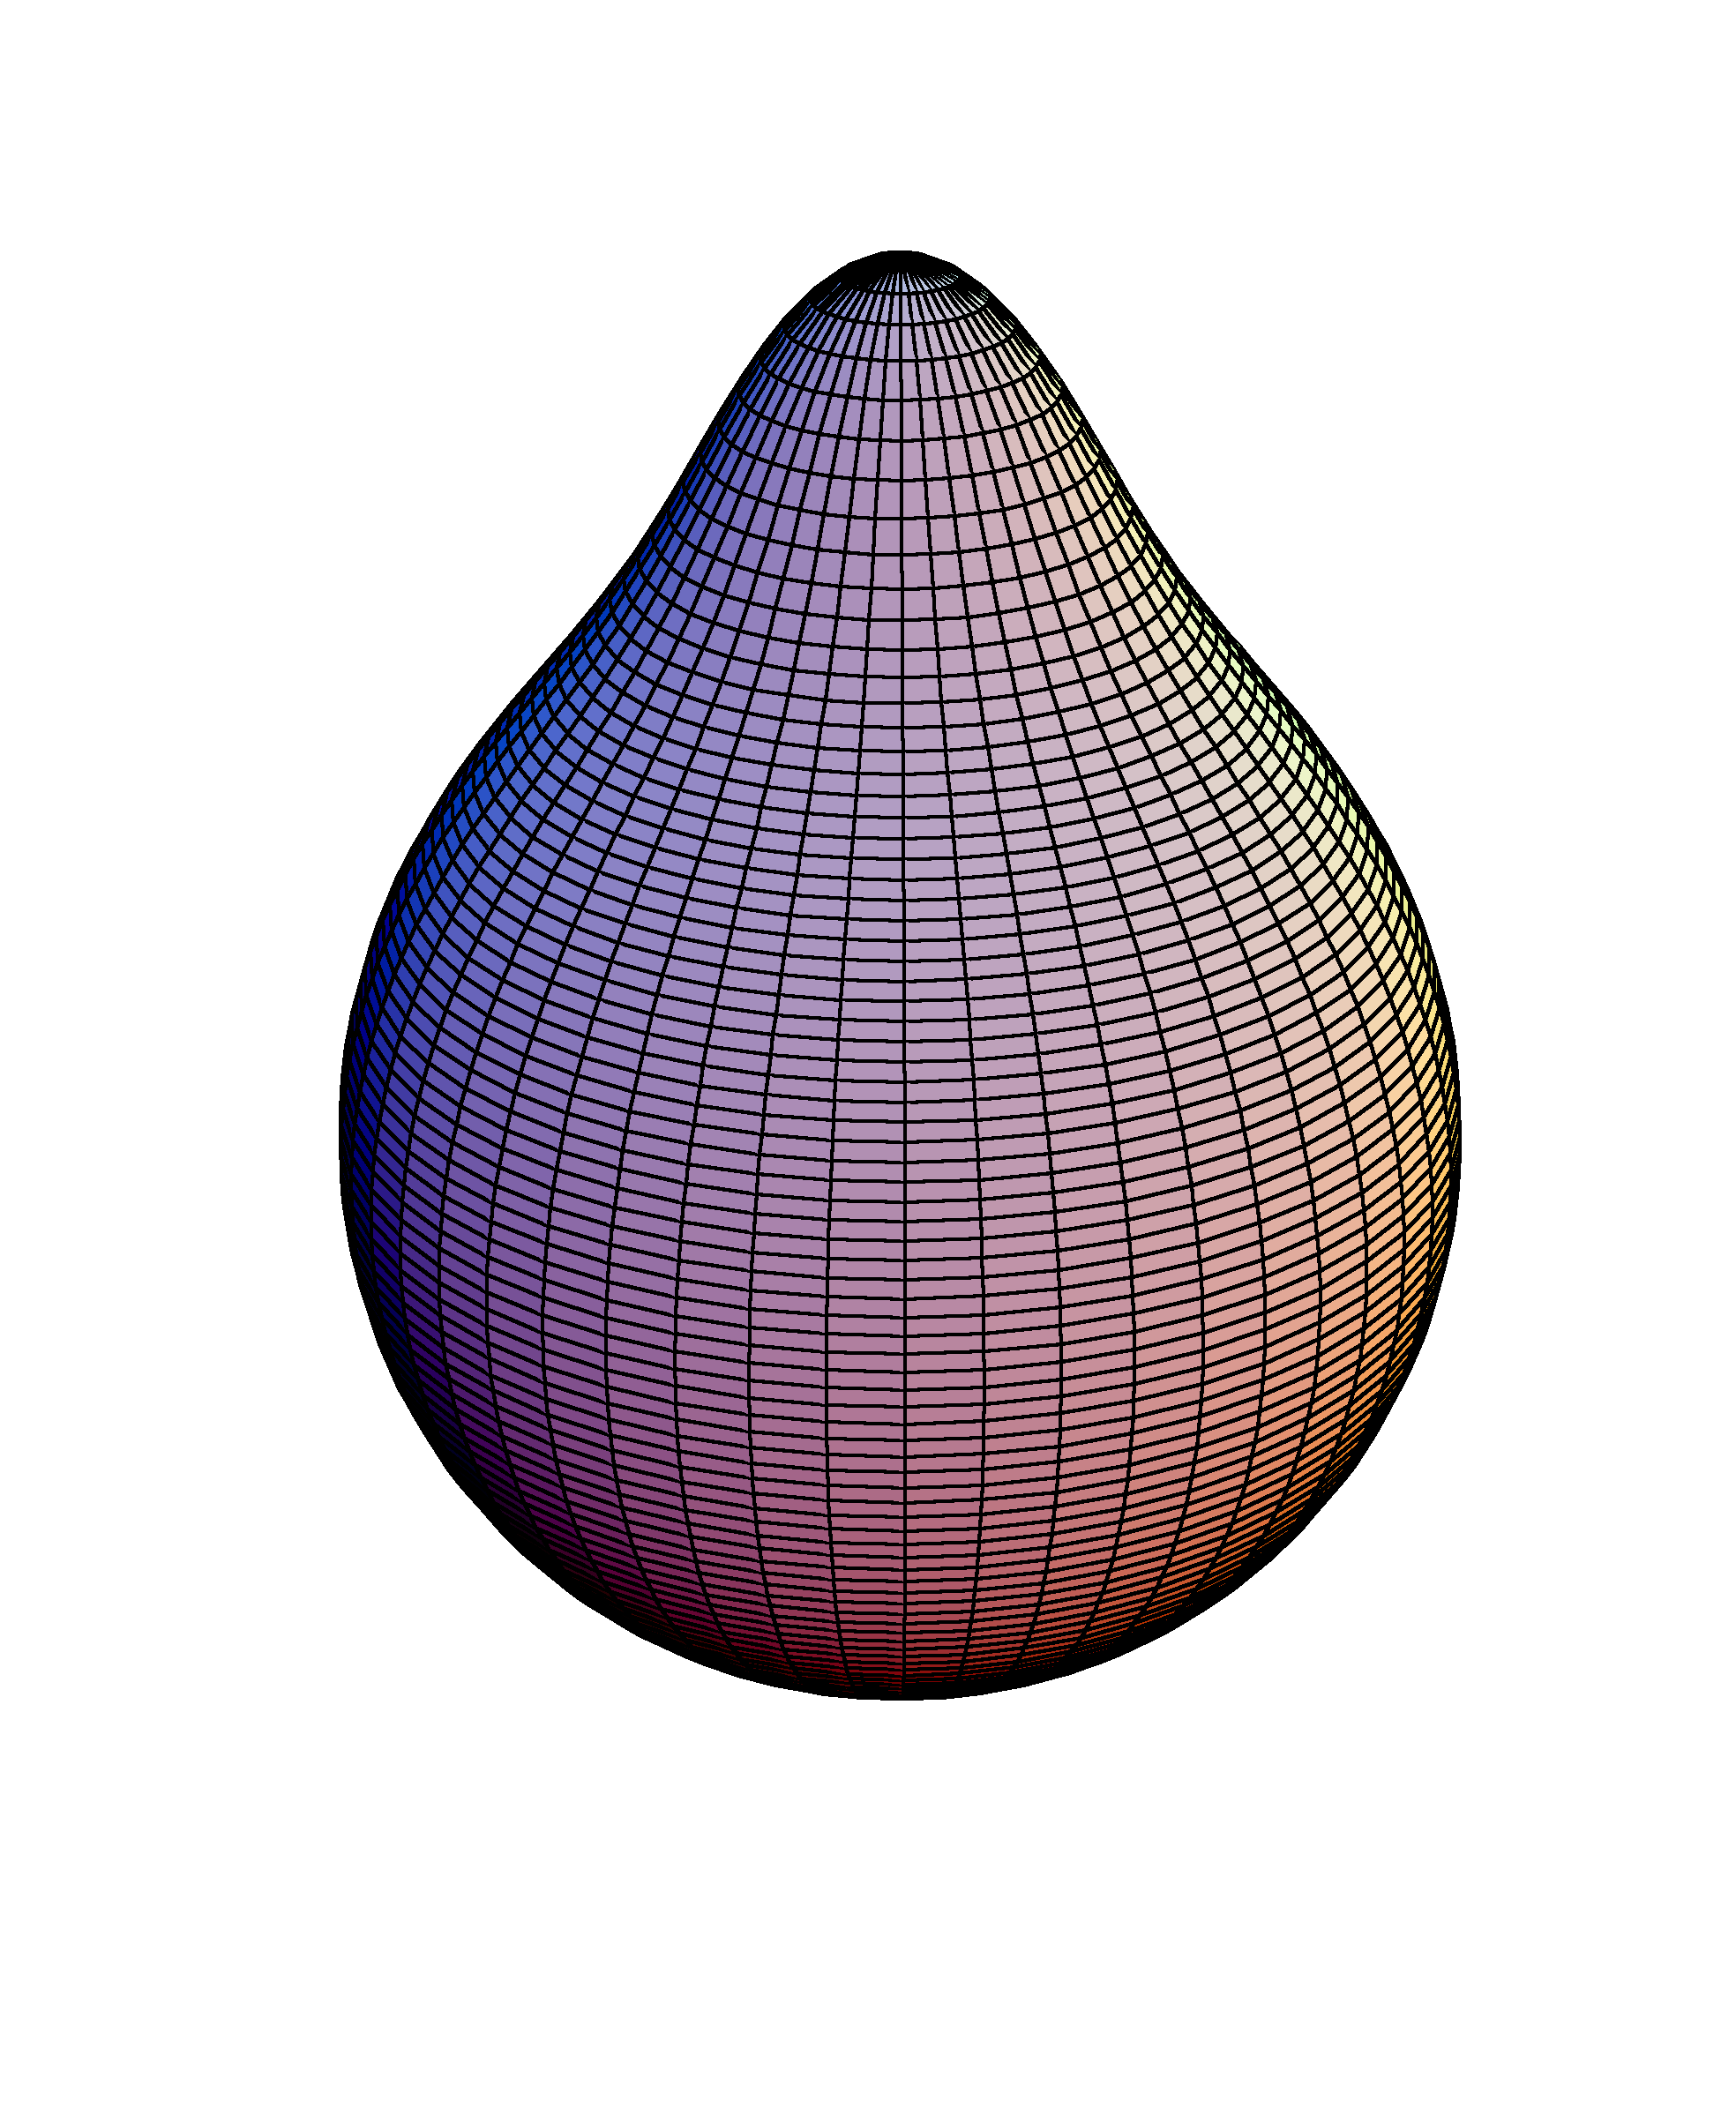
\includegraphics[width=0.5\textwidth]{images/p_070.png}}\hfill
%   \subfigure[$h=0.75$]
%     {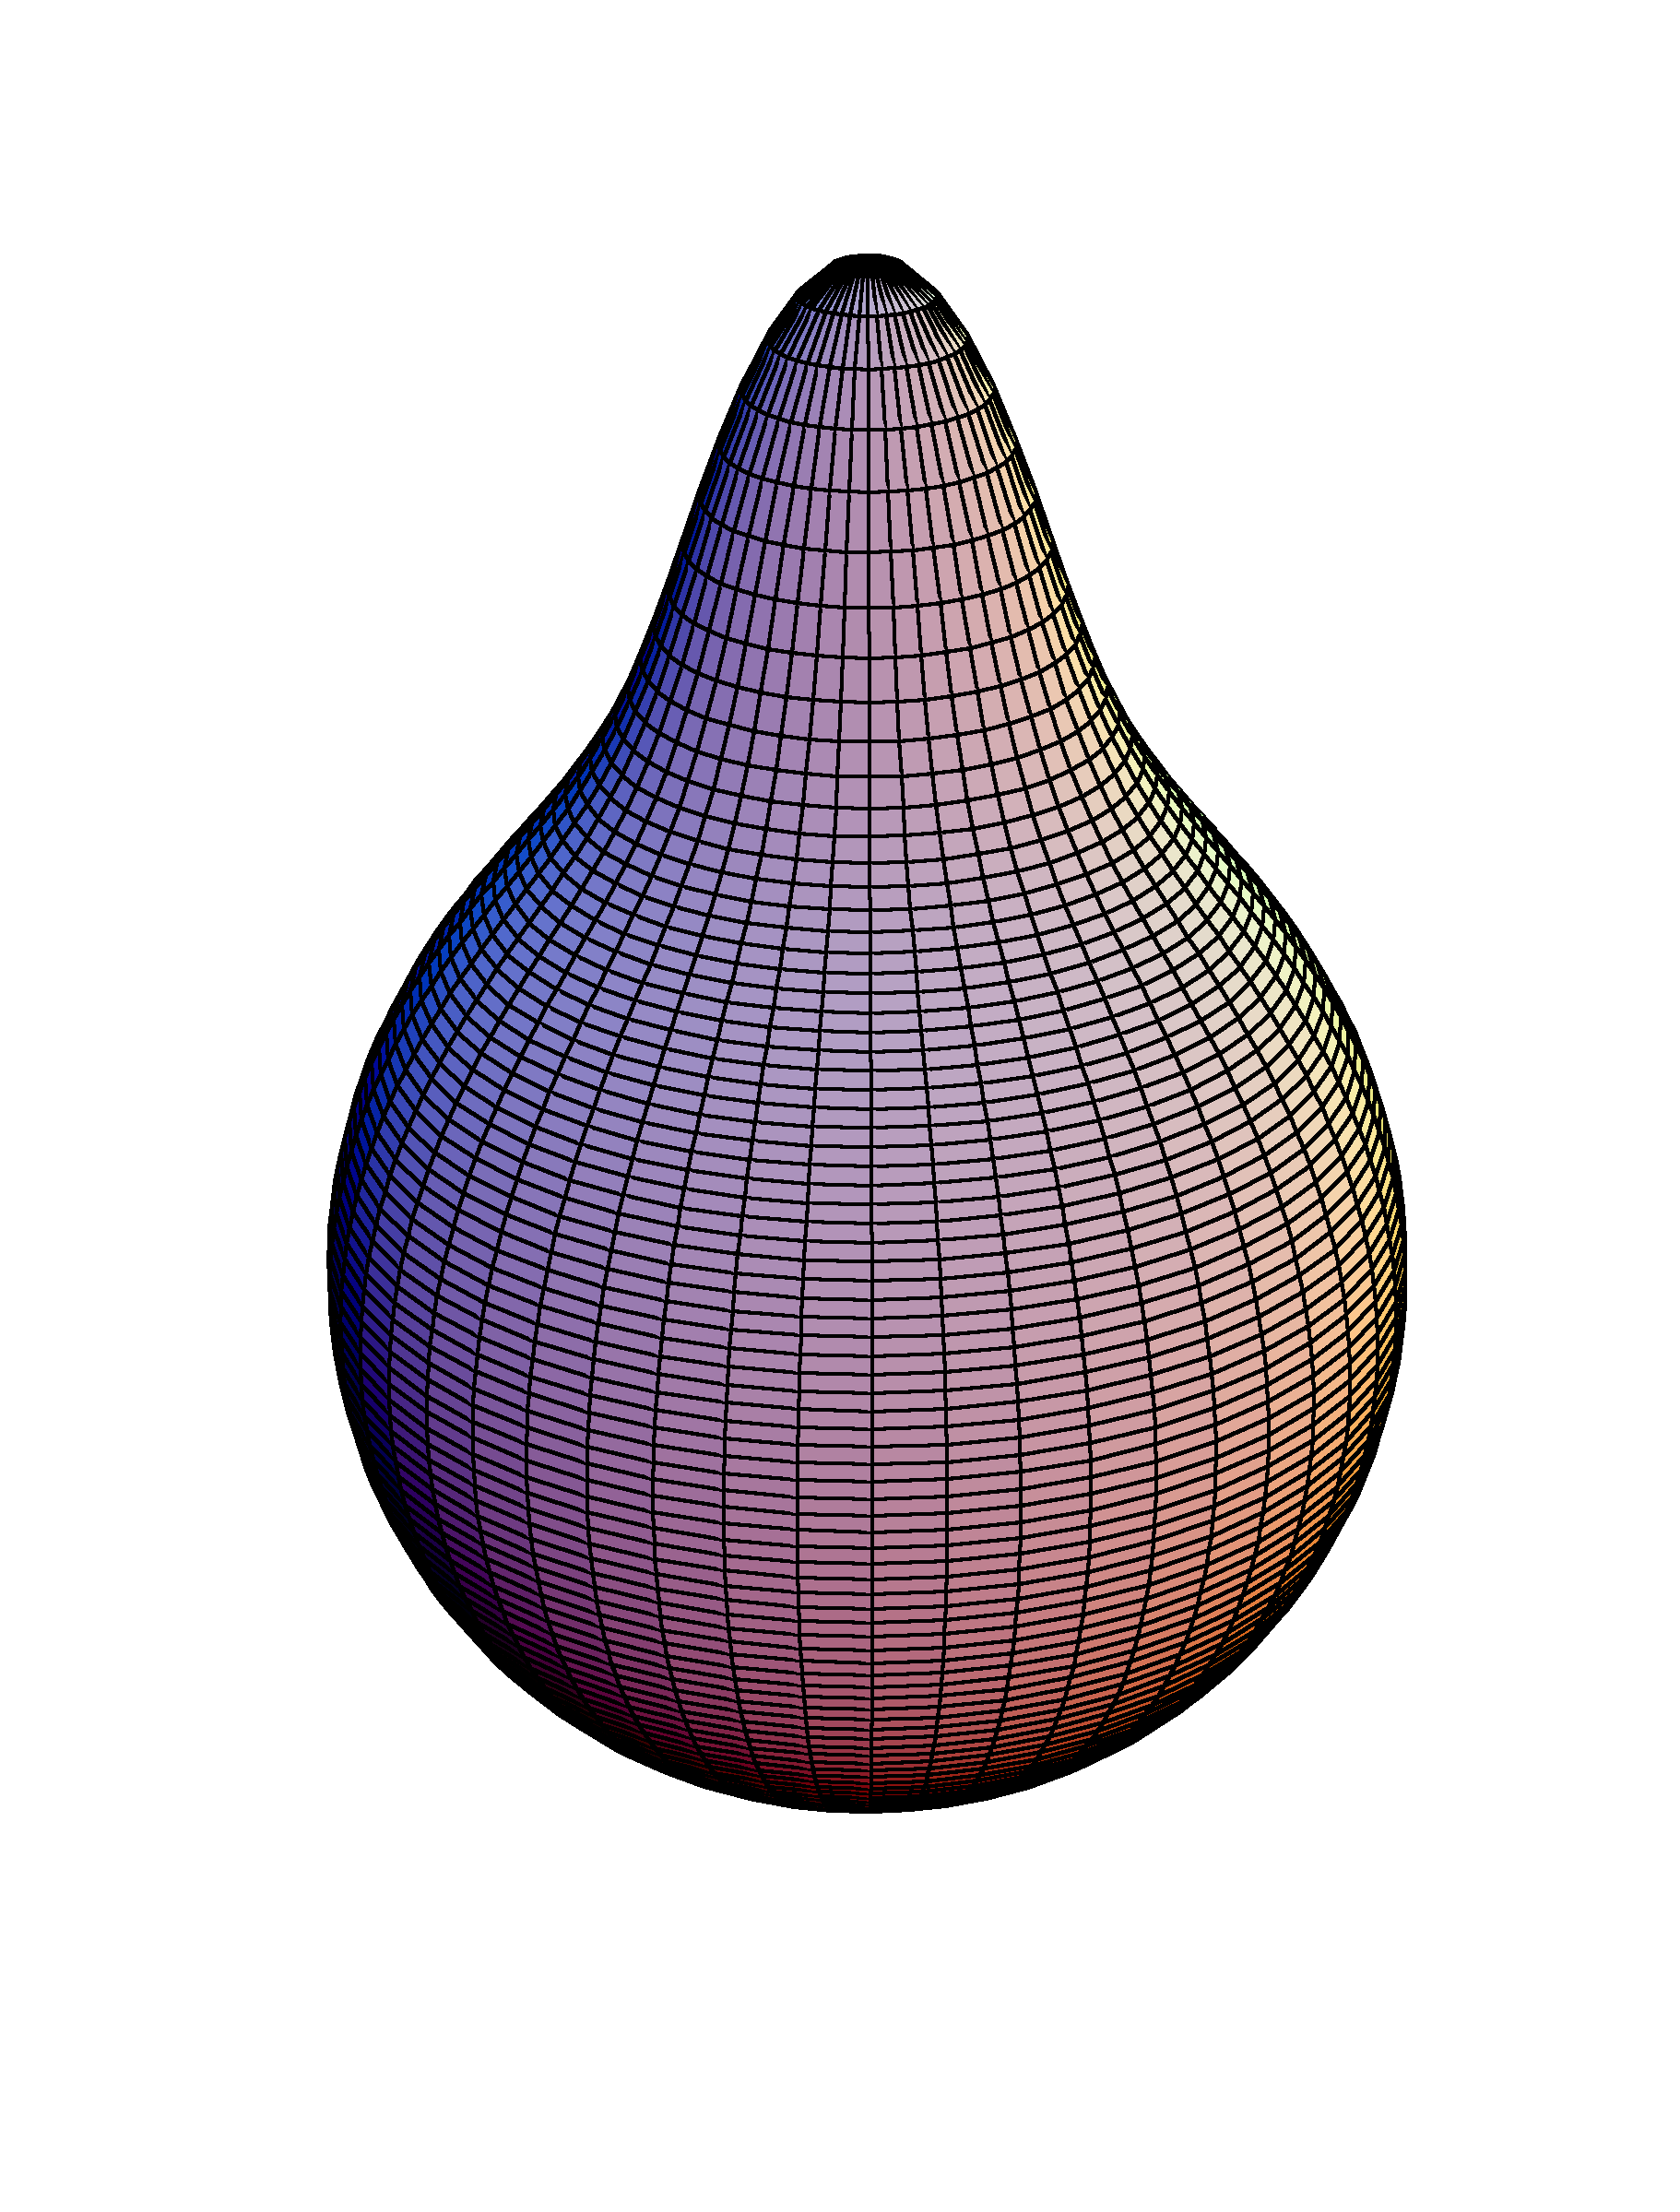
\includegraphics[width=0.5\textwidth]{images/p_075.png}}\\
%   \subfigure[$h=0.80$]
%     {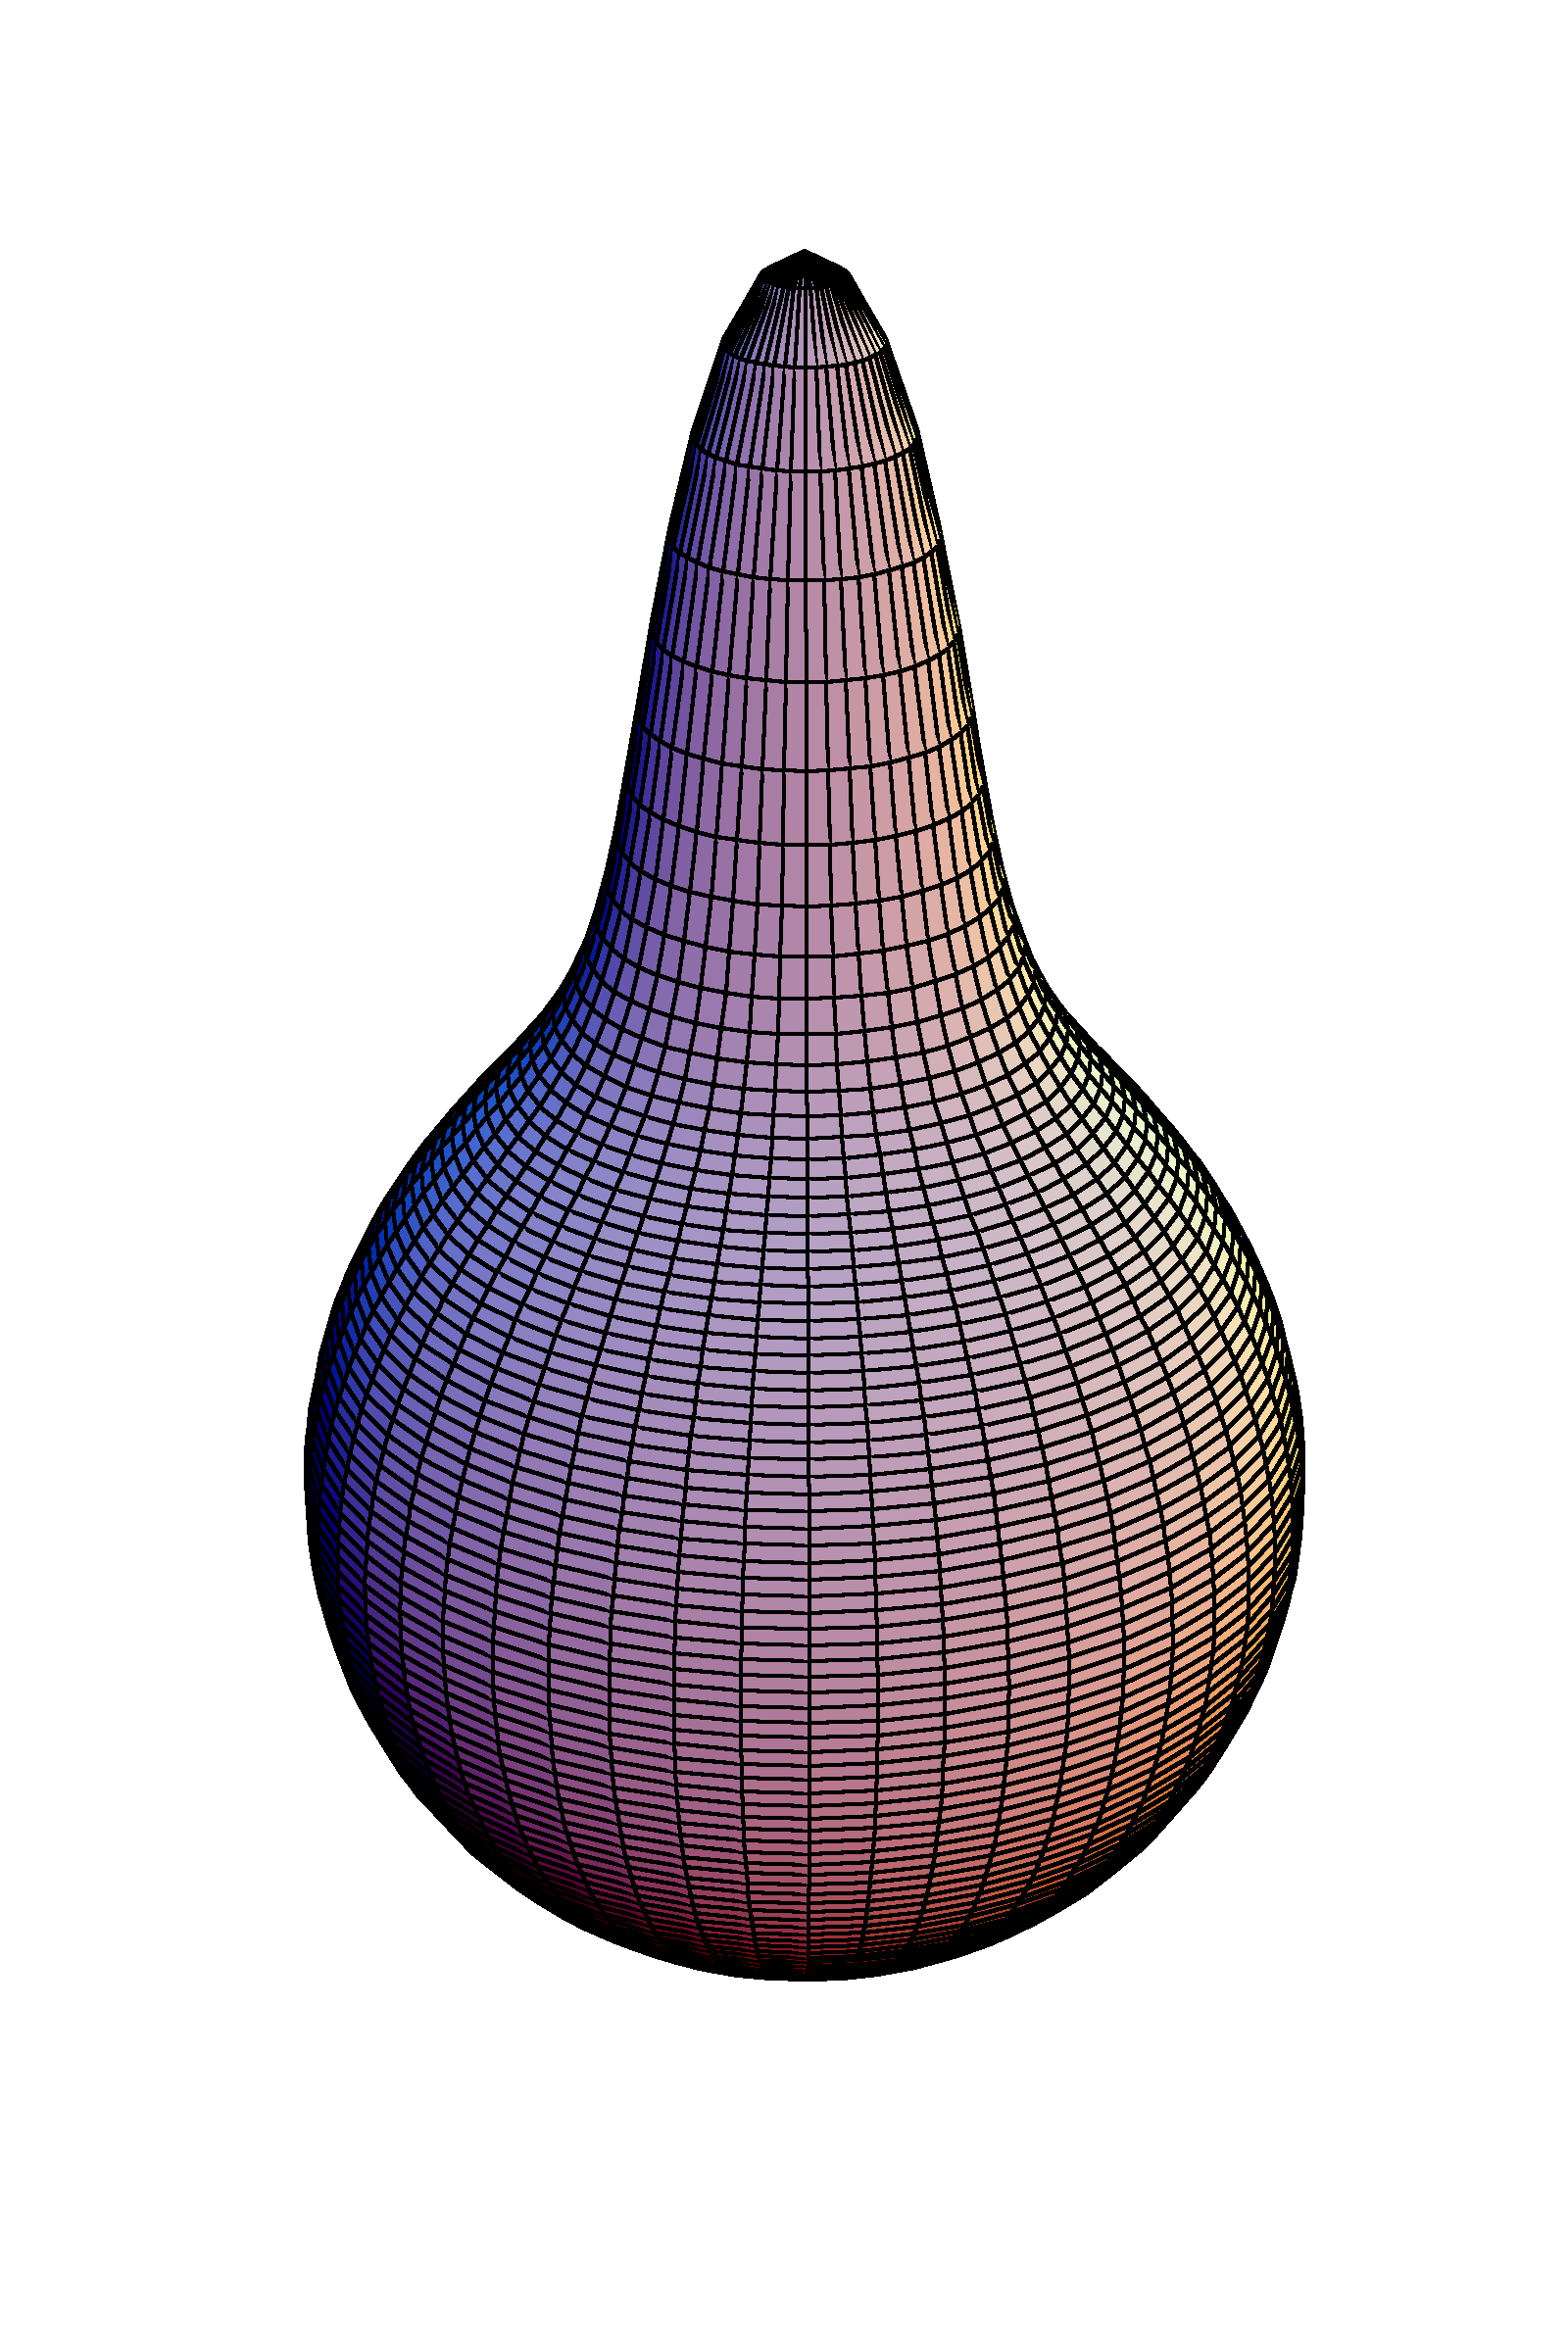
\includegraphics[width=0.5\textwidth]{images/p_080.png}}\hfill
%   \subfigure[$h=0.85$]
%     {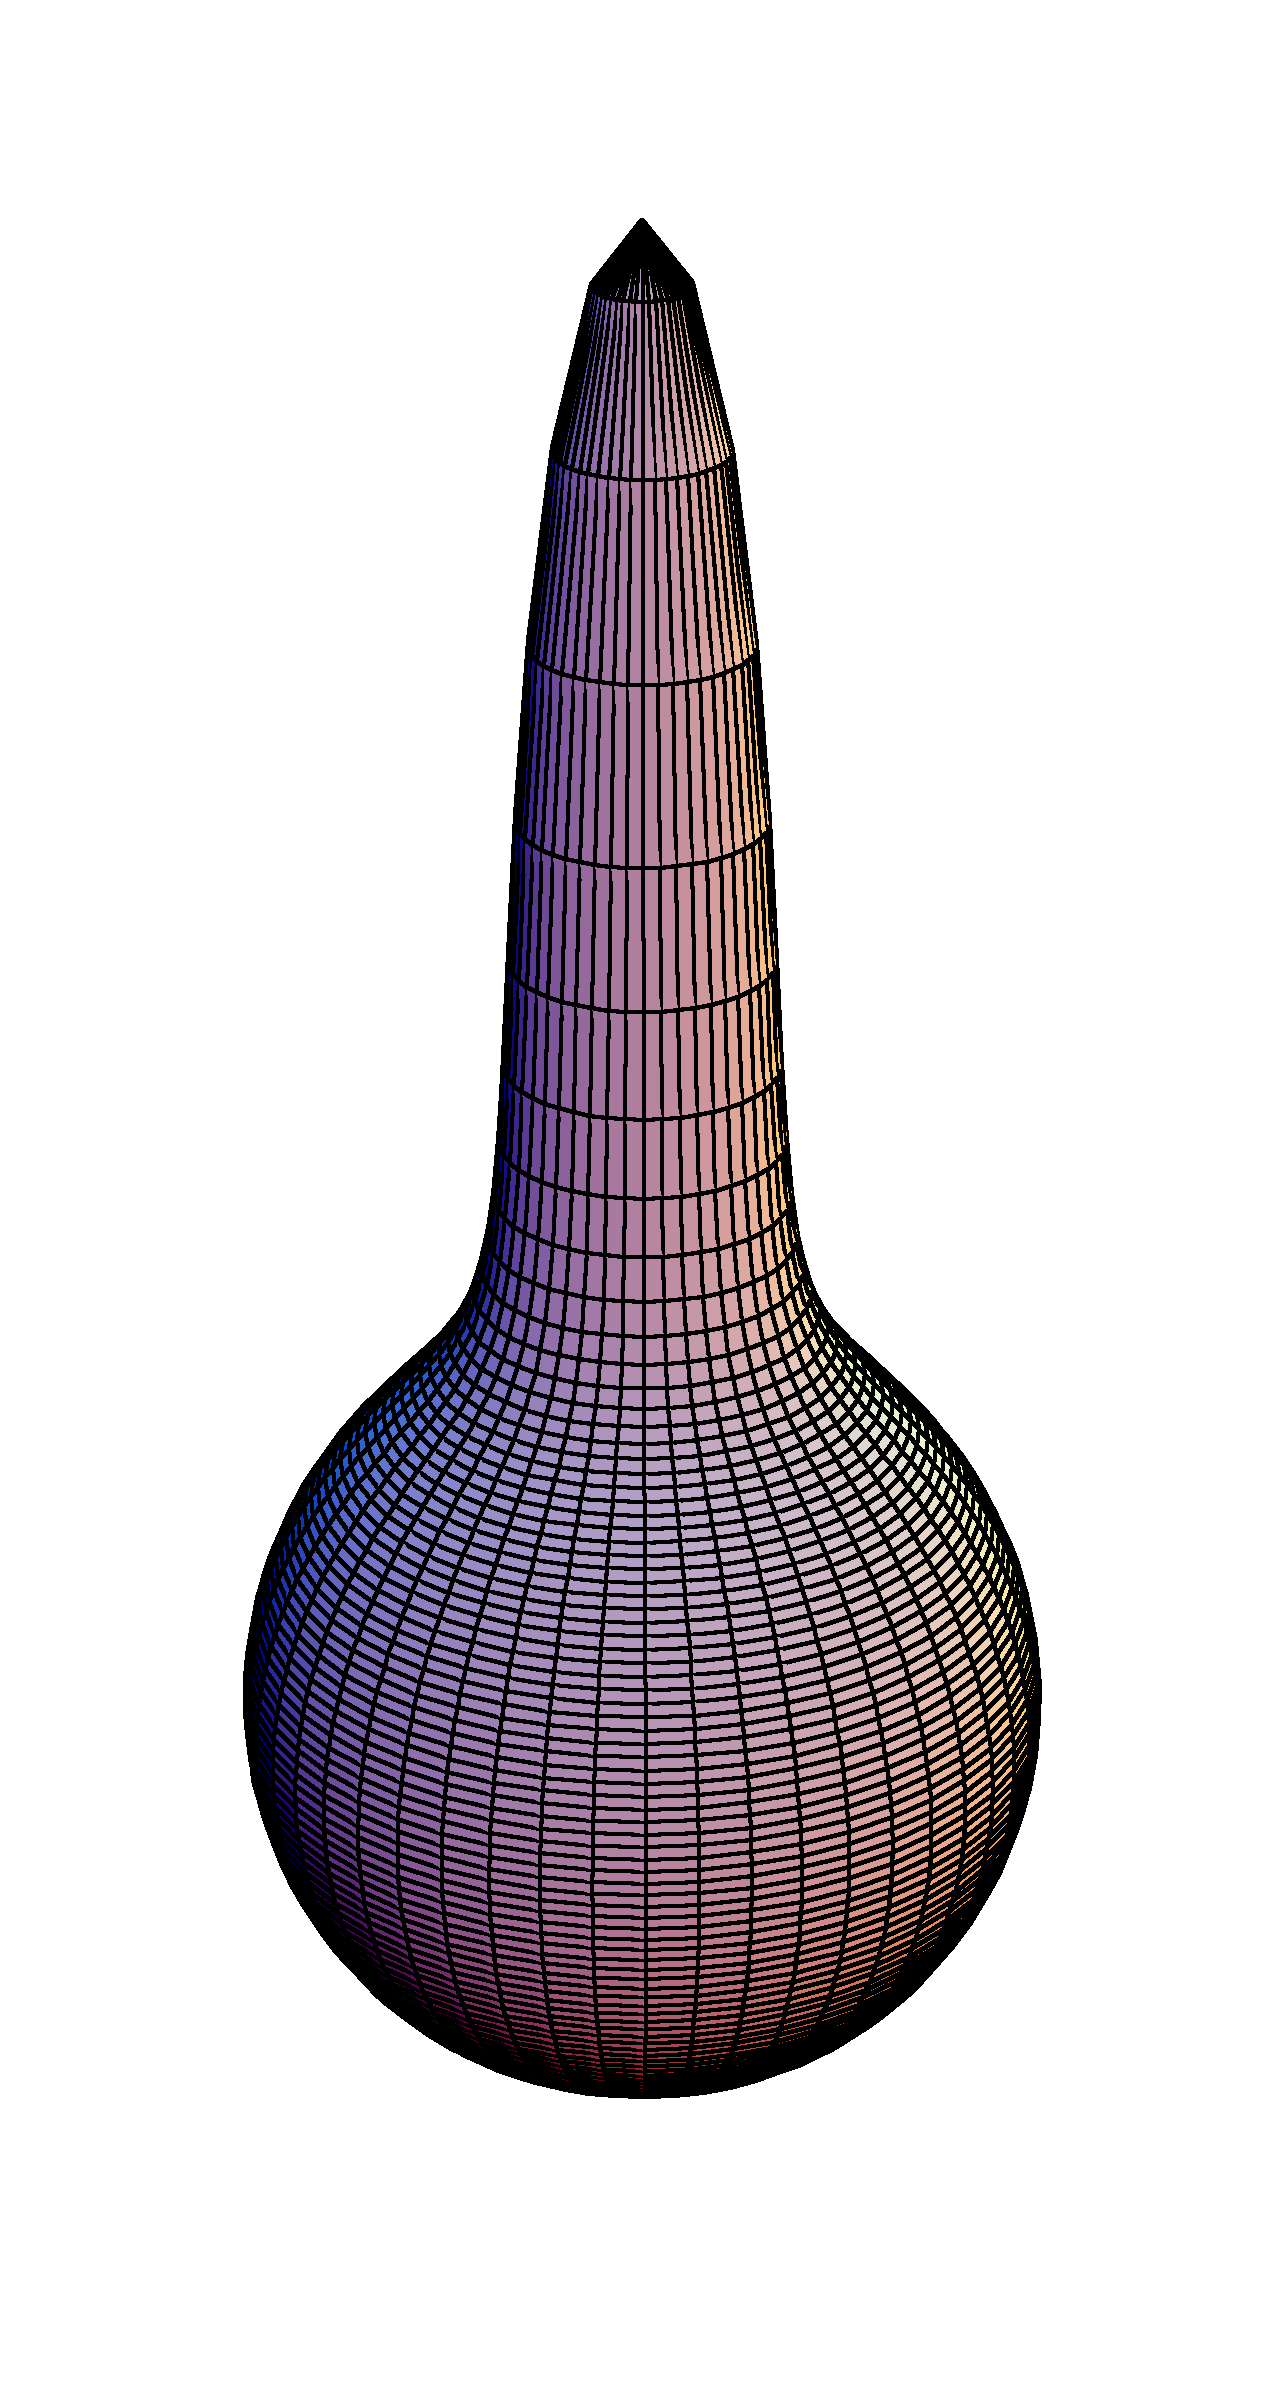
\includegraphics[width=0.5\textwidth]{images/p_085.png}}
%  \caption{The Poisson kernel plotted as a spherical radial basis function on the sphere for different values of $h$.}
%  \label{Basics:Figure:PoissonKernel2}
%\end{figure}

\begin{example}
  We define the \emph{singularity kernel} $S_{h}:\interv{[}{-1}{1}{]} \rightarrow \R$ by
  \[
    \fun{S_{h}}{x} := \frac{1}{2\pi} \frac{1}{\paren{1-2hx+h^2}^{1/2}}  \quad \paren{x \in \interv{[}{-1}{1}{]}}.
  \]
  Using \eqref{Basics:Solution} we obtain
  \[
    \fun{S_{h}}{x} = \sum_{k = 0}^{\infty} \frac{1}{2\pi} h^k \fun{P_k}{x}
  \]
  and therefore
  \[
    \fun{S_{h}^{\wedge}}{k} = \frac{2k+1}{2} h^k.
  \]
  See Figure \ref{Basics:Figure:SingularityKernel} and for more information \cite[pp. 112]{frgesc}.
\end{example}

\begin{figure}[tbp]
  \centering
  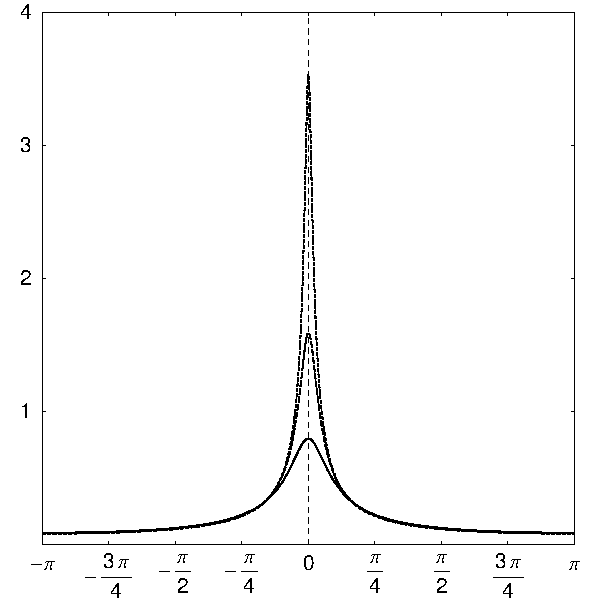
\includegraphics[width=0.7\textwidth]{images/singularity}
  \caption{The singularity kernel $\fun{S_{h}}{\cos\theta}$ for $h = 0.8,0.9,0.95$ and $\theta \in \interv{[}{-\pi}{\pi}{]}$.}
  \label{Basics:Figure:SingularityKernel}
\end{figure}

\begin{example}
  The locally supported kernel $L_{h,\lambda}: \interv{[}{-1}{1}{]} \rightarrow \R$ mentioned in \cite{frsc} and defined by
  \[
    \fun{L_{h,\lambda}}{x} := 
      \left\{\begin{array}{l@{\quad \text{if} \quad}l} 
                                              0 & -1 \le x \le h, \\
        \frac{\lambda+1}{2\pi(1-h)^{\lambda+1}}\paren{x-h}^{\lambda} &  h   < x \le 1,
      \end{array}\right.
  \]
  has the recursively defined symbol $\fun{L_{h,\lambda}^{\wedge}}{k}$ with
\begin{eqnarray*}
    \fun{L_{h,\lambda}^{\wedge}}{0} & = & 1,\\
    \paren{\lambda+1} \fun{L_{h,\lambda}^{\wedge}}{1} & = & \paren{\lambda + 1 + h},\\
    \paren{k+\lambda+2} \fun{L_{h,\lambda}^{\wedge}}{k+1} & = & \paren{2k+1} h \fun{L_{h,\lambda}^{\wedge}}{k} - \paren{k-\lambda-1} \fun{L_{h,\lambda}^{\wedge}}{k-1} 
    \quad \paren{k = 1,2,\ldots}.
\end{eqnarray*}
  Figure \ref{Basics:Figure:LKernel} shows the function $L_{h,\lambda}$ for different values $h$ and $\lambda$.
\end{example}

\begin{figure}[tb]
  \centering
   \subfigure[$\lambda=1.5$]
     {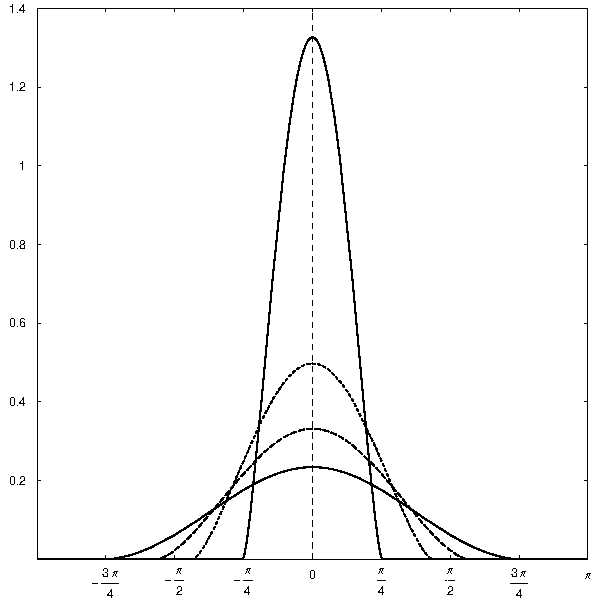
\includegraphics[width=0.33\textwidth]{images/locsup4}}\hfill
   \subfigure[$\lambda=1.0$]
     {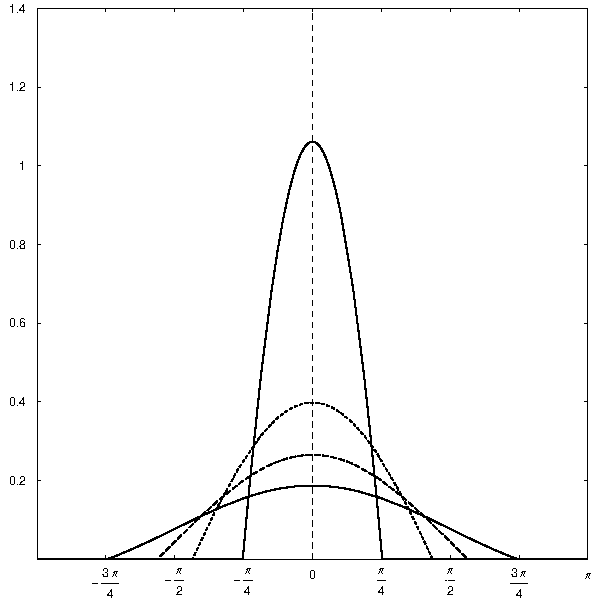
\includegraphics[width=0.33\textwidth]{images/locsup3}}\\
   \subfigure[$\lambda=0.5$]
     {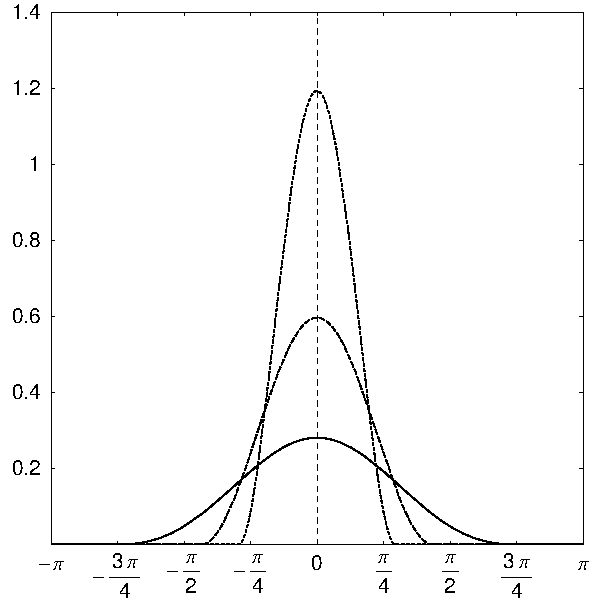
\includegraphics[width=0.33\textwidth]{images/locsup2}}\hfill
   \subfigure[$\lambda=0.2$]
     {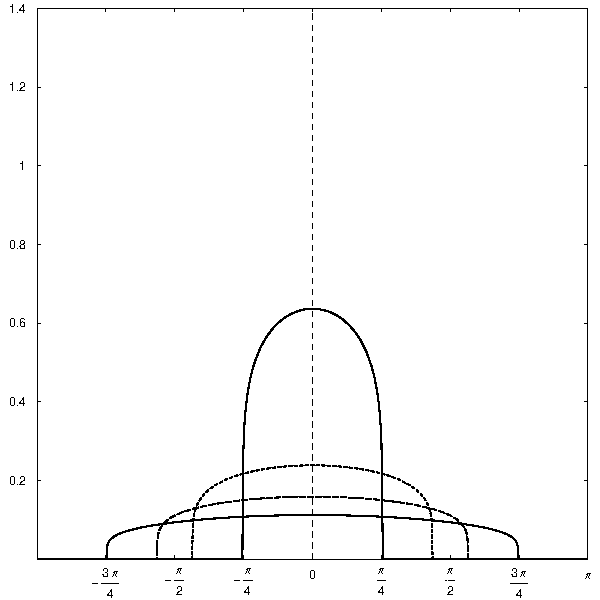
\includegraphics[width=0.33\textwidth]{images/locsup1}}
  \caption{The kernel $L_{h,\lambda}$ for $h = -0.7, -0.2, 0.2, 0.7$ and different values of $\lambda$.}
  \label{Basics:Figure:LKernel}
\end{figure}

\section{Conclusions}



%-----------------------------------------------------------------------------
\bibliographystyle{abbrv}
\bibliography{/home/potts/tex/ref}
%\bibliography{ref}
%\bibliography{../myrefs}
\end{document}
